We can use the fact that every function can be written as a linear combination of the eigenfunctions for the Green's function. We then get
\begin{align*}
  G_D(\vec{x},\vec{y}) = \sum_{n}c_n(\vec{y}) \Psi_n(\vec{x})
\end{align*}
so instead of solving for the Green's function conditions, we solve for the laplace equation and then calculate the coefficients.

Since we want the Green's function to satisfy
\begin{align*}
  \nabla_{\vec{x}}^{2}G_D(\vec{x},\vec{y}) 
  =
  - 4 \pi \delta(\vec{x} - \vec{y})
\end{align*}
so plugging this into the eigenfunction expansion together with the completness, we obtain
\begin{align*}
  \sum_{n}c_n(\vec{y}) \nabla_{\vec{x}}^{2}\Psi(\vec{x}) 
  = 
  \sum_{n}c_n(\vec{y}) \lambda_n \Psi_n(\vec{x}) 
  = 
  - 4 \pi \psi(\vec{x}- \vec{y})
  =
  - 4\pi \sum_{n} \Psi_n^{\ast}(\vec{y}) \Psi_n(\vec{x})
\end{align*}
or equivalently,
\begin{align*}
  \sum_{n} \left[
    c_n(\vec{y}) \lambda_n + 4 \pi \Psi_n^{\ast}(\vec{y})
  \right]
  \Psi_n(\vec{x})
  = 0
\end{align*}
which can only be zero if the coefficients are all zero, so it must be that for each $n$ we have
\begin{align*}
  c_n(\vec{y}) = - \frac{4 \pi}{\lambda_n} \Psi_n^{\ast}(\vec{y}))
\end{align*}

Putting this together we get a recipe to find the Green's function:
\begin{empheq}[box=\bluebase]{align*}
G_D(\vec{x},\vec{y}) = - 4 \pi \sum_{n} \frac{\Psi_n^{\ast}(\vec{y})\Psi_n(\vec{x})}{\lambda_n}
\end{empheq}


However, this is all under the assumption that the eigenstates showed no degeneracy.
But we obvioulsy know since the eigenvalues are energy, they are degenerate as multiple states can have the same energy and we \emph{might} not have orthogonality and completeness.

There is a way around this. If instead of solving for laplace eigenfunctions , we solve for eigenfunctions of the momentum operator
\begin{align*}
  \hat{p} \Psi_n = \vec{\nabla} \Psi_n = \vec{p}_n \vec{\Psi}
\end{align*}
we see that there is no degeneracy here.

\begin{ex}[Sanity check]
  We want to find the Green's function $G_D(\vec{x},\vec{y})$ with no boundary conditions. We know the answer, as it is simply 
  \begin{align*}
    G_D(\vec{x},\vec{y}) = \frac{1}{\abs{\vec{x}- \vec{y}}}
  \end{align*}
  Let's to use our new laplace eigenfunction method and see if it produces the right result.
  Before we solve the laplace equation, we first solve for the momentum eigenstate:
  \begin{align*}
    \vec{\nabla}\Psi(\vec{x}) = i \vec{p} \Psi(\vec{x})
  \end{align*}
  That is very easy as we can just solve the first order ODE for each component of $\Psi$.
  The eigenfunction is then given by
  \begin{align*}
    \Psi_{\vec{p}}(\vec{x}) = \frac{1}{(2 \pi)^{3/2}}e^{i \vec{p}\bm{\cdot} \vec{x}}
  \end{align*}
  so for the laplacian, the we get the eigenfunctions 
  \begin{align*}
    \nabla^{2} \Psi_{\vec{p}}(\vec{x}) = -p^{2} \Psi_{\vec{p}}(\vec{x})
  \end{align*}
  Now, we check for orthogonality and completness:
  \begin{align*}
    \int d^{3}\vec{x} \Psi_{\vec{p}}^{\ast}(\vec{x}) \Psi_{\vec{k}}(\vec{x}) 
    &= 
    \int d^{3}\vec{x} \frac{1}{(2 \pi)^{3}}e^{-i \vec{p} \bm{\cdot} \vec{x}} e^{+ i \vec{k} \bm{\cdot} \vec{x}}
    \\
    &= \int d^{3} \vec{x} \frac{1}{(2 \pi)^{3}} e^{-i(\vec{p}- \vec{k})\bm{\cdot} \vec{x}}
    \\
    &=
    \delta(\vec{p} - \vec{k})
  \end{align*}
  where we used the fact from MMP-I that the fourier transform of the identity is the delta function.

  For completeness, our eigenfunctions are indexed by a continuous variable $\vec{p}$, so we need to calculate
  \begin{align*}
    \int d^{3}\vec{k} \Psi_{\vec{k}}^{\ast}(\vec{x}) \Psi_{\vec{k}}(\vec{y})
    =
    \int d^{3}\vec{k} \frac{1}{(2 \pi)^{3}} e^{-i \vec{k} \bm{\cdot}(\vec{x}- \vec{y}} 
    = 
    \delta(\vec{x}-\vec{y})
  \end{align*}
  So our Eigenfunctions are indeed both orthonormal and complete.
  Now we can use our recipe to find the Green's function:
  \begin{align*}
    G_D(\vec{x},\vec{y}) 
    &= 
    - 4 \pi \int d^{3}\vec{k} \frac{\Psi_{\vec{k}}^{\ast}(\vec{y})\Psi_{\vec{k}}(\vec{x})}{\lambda_n}
    \\
    &=
    - 4 \pi \int d^{3}\vec{k} \frac{1}{(2 \pi)^{3}} \frac{e^{-i \vec{k} \bm{\cdot}(\vec{y} - \vec{x}}}{- \abs{\vec{k}}^{2}}\\
    &= \frac{1}{\abs{\vec{x} - \vec{y}}}
  \end{align*}
  where in the last step we used the fourier transform from MMP-I.
\end{ex}
For such a simple problem the Laplace method may seem overkill, but we can solve the electrostatic problem for various situations.
\begin{ex}[Electrostatics in a box]
In this example, we have a box with sidelengths $a,b,c$ and we want a Green's function for a solution $\Psi$ that vanishes on the
$\pi a \rho a \lambda \eta \lambda \epsilon \pi i \pi \epsilon \delta \sigma$

A solution we have derived in Physics III is 
\begin{align*}
  \Psi_{lmn}(\vec{x}) = \sqrt{\frac{8}{abc}} \sin \frac{l \pi x}{a} \sin \frac{m \pi y}{b} \sin \frac{n \pi z}{c}
\end{align*}
which satisfies the boundary condtion and is an eigenfunction of the laplace equation
\begin{align*}
  \nabla^{2}\Psi_{lmn}(\vec{x}) = - \pi \left(
    \frac{l^{2}}{a^{2}}+ \frac{m^{2}}{b^{2}}+ \frac{n^{2}}{c^{2}}
  \right)  
  \Psi_{lmn}(\vec{x})
\end{align*}
This time, the eigenfunctions are discrete and we can also show orthogonality and completeness (but that is now shown here)

Then, the Green's function is given by
\begin{align*}
  G_D(\vec{x}, \vec{y})
  &=
  - \pi
  \sum_{n,l,m} \frac{\Psi_{lmn}^{\ast}(\vec{x})\Psi_{lmn}(\vec{y})}{\lambda_{lmn}}
\end{align*}
which cannot really be simplified any further. They belong to a family called \textbf{hypergeometric functions}
\end{ex}

\begin{figure}[h]
\centering
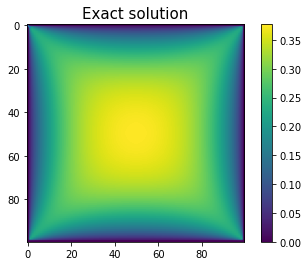
\includegraphics[width=0.5\textwidth]{./img/2d-paralelepipeds.png}
\caption{Plot of the Potential $\Phi$ for the 2-D square paralelepipeds}
\end{figure}

